\documentclass[11pt]{article}

\usepackage[margin=1in]{geometry}
\usepackage{setspace}
\onehalfspacing
\usepackage{graphicx}
\graphicspath{report_images/}
\usepackage{appendix}
\usepackage{listings}
\usepackage{float}
\usepackage{multirow}
\usepackage{amsthm}
% The next three lines make the table and figure numbers also include section number
\usepackage{chngcntr}
\counterwithin{table}{section}
\counterwithin{figure}{section}
% Needed to make titling page without a page number
\usepackage{titling}

% This section required for the code block stuff below
\usepackage{color}
\definecolor{codegreen}{rgb}{0,0.6,0}
\definecolor{codegray}{rgb}{0.5,0.5,0.5}
\definecolor{codepurple}{rgb}{0.58,0,0.82}
\definecolor{backcolour}{rgb}{0.95,0.95,0.92}

% Makes code blocks have shaded backgrounds and line numbers
\lstdefinestyle{mystyle}{
    backgroundcolor=\color{backcolour},   
    commentstyle=\color{codegreen},
    keywordstyle=\color{magenta},
    numberstyle=\tiny\color{codegray},
    stringstyle=\color{codepurple},
    basicstyle=\footnotesize,
    breakatwhitespace=false,         
    breaklines=true,                 
    captionpos=b,                    
    keepspaces=true,                 
    numbers=left,                    
    numbersep=5pt,                  
    showspaces=false,                
    showstringspaces=false,
    showtabs=false,                  
    tabsize=2
}
 
\lstset{style=mystyle}

% DOCUMENT INFORMATION =================================================
\font\titleFont=cmr12 at 11pt
\title {{\titleFont ECEN 424: Advanced Digital Design\\ North Carolina Agricultural and Technical State University \\ Department of Electrical and Computer Engineering}} % Declare Title
\author{\titleFont Chris Cannon} % Declare authors
\date{\titleFont 2018-12-05}
% ======================================================================

\begin{document}

\begin{titlingpage}
\maketitle
\begin{center}
	Project 2 Report \\ Rev. 1.0.2
\end{center}
\end{titlingpage}

\tableofcontents

\pagebreak

\section{System Overview}
This system will be a VHDL-based digital lock that must be implemented on the Digilent Basys3 FPGA. The lock will take a 6-digit code, entered via a standard USB numeric keyboard. The code must be re-programmable. The system must notify a user of an incorrect password and must lock permanently after 3 incorrect attempts.

\section{Modules}

\subsection{Module Overview}

The system should include the following modules

\begin{table}[H]
\begin{tabular}{| p{5cm} | p{10.5cm} |}
	\hline
	Module & Description \\ \hline
	digital\textunderscore lock & Top-level that includes all other modules \\ \hline
	main & Main finite state machine \\ \hline
	code\textunderscore timeout\textunderscore timer & Counts to 20 seconds, after which it will notify the main so that the code can be cleared. \\ \hline
	set\textunderscore timeout\textunderscore timer & Counts to 10 seconds, after which it will notify the main so that the set state can be exited \\ \hline
	open\textunderscore timeout\textunderscore timer & Counts to 15 seconds, after which it will notify the main to lock the system \\ \hline
	display\textunderscore timeout\textunderscore timer & Counts to 5 seconds, after which it will notify the display-controller so that the display will be cleared \\ \hline
	clock\textunderscore divider & Divides the clock signal to 1 Hz \\ \hline
	input\textunderscore controller & Interprets the keystrokes from the USB keyboard and passes the appropriate command to the main\\ \hline
	debouncer & Prevent input signal from bouncing too rapidly, creating incorrect input \\ \hline
	output\textunderscore controller & Interprets the command from main and displays the appropriate message on the VGA display and LED \\ \hline
\end{tabular}
\end{table}

\subsection{main}

\subsection{Overview}

The main module is the finite state machine that controls all other components in digital\textunderscore lock.

\subsubsection{Inputs}

\begin{table}[H]
\begin{tabular}{| p{2.5cm} | p{6cm} | p{6cm} |}
	\hline
	Input Name & Data Type & Description \\ \hline
	cmd & std\textunderscore logic\textunderscore vector(3 downto 0) & Input command from the input\textunderscore controller module. \\ \hline
	code\textunderscore timeout & std\textunderscore logic & Indicates when the code entry has timed out. \\ \hline
	set\textunderscore timeout & std\textunderscore logic & Indicates when the set function has timed out. \\ \hline
	open\textunderscore timeout & std\textunderscore logic & Indicates when the lock should close. \\ \hline
	clk & std\textunderscore logic & Board clock signal \\ \hline
\end{tabular}
\end{table}

\subsubsection{Outputs}

\begin{table}[H]
\begin{tabular}{| p{2.5cm} | p{6cm} | p{6cm} |}
	\hline
	Output Name & Data Type & Description \\ \hline
	enable\textunderscore code & std\textunderscore logic & Activates the code\textunderscore timeout\textunderscore timer module. \\ \hline
	reset\textunderscore code & std\textunderscore logic & Restarts the code\textunderscore timeout\textunderscore timer module. \\ \hline
	enable\textunderscore set & std\textunderscore logic & Activates the set\textunderscore timeout\textunderscore timer module. \\ \hline
	reset\textunderscore set & std\textunderscore logic & Restarts the set\textunderscore timeout\textunderscore timer module. \\ \hline
	enable\textunderscore open & std\textunderscore logic & Activates the open\textunderscore timeout\textunderscore timer module. \\ \hline
	reset\textunderscore open & std\textunderscore logic & Restarts the open\textunderscore timeout\textunderscore timer module. \\ \hline
	display\textunderscore cmd & std\textunderscore logic\textunderscore vector(3 downto 0) & Binary encoded message for the output\textunderscore controller module. \\ \hline
\end{tabular}
\end{table}

\subsection{code\textunderscore timeout\textunderscore timer}

\subsubsection{Inputs}

\begin{table}[H]
\begin{tabular}{| p{2.5cm} | p{6cm} | p{6cm} |}
	\hline
	Input Name & Data Type & Description \\ \hline
	enable & std\textunderscore logic & Activates the code\textunderscore timeout\textunderscore timer module. \\ \hline
	reset & std\textunderscore logic & Restarts the code\textunderscore timeout\textunderscore timer module. \\ \hline
	clk & std\textunderscore logic & Board clock signal \\ \hline
\end{tabular}
\end{table}

\subsubsection{Outputs}

\begin{table}[H]
\begin{tabular}{| p{2.5cm} | p{6cm} | p{6cm} |}
	\hline
	Output Name & Data Type & Description \\ \hline
	done & std\textunderscore logic & Indicates when the code entry has timed out. \\ \hline
\end{tabular}
\end{table}

\subsection{set\textunderscore timeout\textunderscore timer}

\subsubsection{Inputs}

\begin{table}[H]
\begin{tabular}{| p{2.5cm} | p{6cm} | p{6cm} |}
	\hline
	Input Name & Data Type & Description \\ \hline
	enable & std\textunderscore logic & Activates the set\textunderscore timeout\textunderscore timer module. \\ \hline
	reset & std\textunderscore logic & Restarts the set\textunderscore timeout\textunderscore timer module. \\ \hline
	clk & std\textunderscore logic & Board clock signal \\ \hline
\end{tabular}
\end{table}

\subsubsection{Outputs}

\begin{table}[H]
\begin{tabular}{| p{2.5cm} | p{6cm} | p{6cm} |}
	\hline
	Output Name & Data Type & Description \\ \hline
	done & std\textunderscore logic & Indicates when the set operation has timed out. \\ \hline
\end{tabular}
\end{table}

\subsection{open\textunderscore timeout\textunderscore timer}

\subsubsection{Inputs}

\begin{table}[H]
\begin{tabular}{| p{2.5cm} | p{6cm} | p{6cm} |}
	\hline
	Input Name & Data Type & Description \\ \hline
	enable & std\textunderscore logic & Activates the open\textunderscore timeout\textunderscore timer module. \\ \hline
	reset & std\textunderscore logic & Restarts the open\textunderscore timeout\textunderscore timer module. \\ \hline
	clk & std\textunderscore logic & Board clock signal \\ \hline
\end{tabular}
\end{table}

\subsubsection{Outputs}

\begin{table}[H]
\begin{tabular}{| p{2.5cm} | p{6cm} | p{6cm} |}
	\hline
	Output Name & Data Type & Description \\ \hline
	done & std\textunderscore logic & Indicates when the open state has timed out. \\ \hline
\end{tabular}
\end{table}

\subsection{display\textunderscore timeout\textunderscore timer}

\subsubsection{Inputs}

\begin{table}[H]
\begin{tabular}{| p{2.5cm} | p{6cm} | p{6cm} |}
	\hline
	Input Name & Data Type & Description \\ \hline
	enable & std\textunderscore logic & Activates the display\textunderscore timeout\textunderscore timer module. \\ \hline
	reset & std\textunderscore logic & Restarts the display\textunderscore timeout\textunderscore timer module. \\ \hline
	clk & std\textunderscore logic & Board clock signal \\ \hline
\end{tabular}
\end{table}

\subsubsection{Outputs}

\begin{table}[H]
\begin{tabular}{| p{2.5cm} | p{6cm} | p{6cm} |}
	\hline
	Output Name & Data Type & Description \\ \hline
	done & std\textunderscore logic & Indicates when the display shown has timed out. \\ \hline
\end{tabular}
\end{table}

\subsection{clock\textunderscore divider}

\subsubsection{Inputs}

\begin{table}[H]
\begin{tabular}{| p{2.5cm} | p{6cm} | p{6cm} |}
	\hline
	Input Name & Data Type & Description \\ \hline
	clk & std\textunderscore logic & Board clock signal \\ \hline
\end{tabular}
\end{table}

\subsubsection{Outputs}

\begin{table}[H]
\begin{tabular}{| p{2.5cm} | p{6cm} | p{6cm} |}
	\hline
	Output Name & Data Type & Description \\ \hline
	button\textunderscore clock & std\textunderscore logic & Reduced 4 Hz clock signal for the input\textunderscore controller module. \\ \hline
\end{tabular}
\end{table}

\subsection{input\textunderscore controller}

\subsubsection{Inputs}

\begin{table}[H]
\begin{tabular}{| p{2.5cm} | p{6cm} | p{6cm} |}
	\hline
	Input Name & Data Type & Description \\ \hline
	PS2Data & variable & Data stream from the USB keyboard. \\ \hline
	clk & std\textunderscore logic & Board clock signal \\ \hline
\end{tabular}
\end{table}

\subsubsection{Outputs}

\begin{table}[H]
\begin{tabular}{| p{2.5cm} | p{6cm} | p{6cm} |}
	\hline
	Output Name & Data Type & Description \\ \hline
	cmd & std\textunderscore logic\textunderscore vector(3 downto 0) & Command-code to for main method based on the input received. \\ \hline
\end{tabular}
\end{table}

\subsection{debouncer}

\subsubsection{Inputs}

\begin{table}[H]
\begin{tabular}{| p{2.5cm} | p{6cm} | p{6cm} |}
	\hline
	Input Name & Data Type & Description \\ \hline
	clk & std\textunderscore logic & The board clock signal \\ \hline
	button & std\textunderscore logic & The signal to be debounced \\ \hline
	button
\end{tabular}
\end{table}

\subsubsection{Outputs}

\begin{table}[H]
\begin{tabular}{| p{2.5cm} | p{6cm} | p{6cm} |}
	\hline
	Output Name & Data Type & Description \\ \hline
	result & std\textunderscore logic & The debounced signal \\ \hline
\end{tabular}
\end{table}

\subsection{output\textunderscore controller}

\subsubsection{Inputs}

\begin{table}[H]
\begin{tabular}{| p{2.5cm} | p{6cm} | p{6cm} |}
	\hline
	Input Name & Data Type & Description \\ \hline
	display & std\textunderscore logic\textunderscore vector(3 downto 0) & Binary encoded message to display on VGA display and lockdown LED \\ \hline
	timeout & std\textunderscore logic & Notifies the controller that the maximum display time has been reached and it should clear any message except "OPEN" \\ \hline
	clk & std\textunderscore logic & Board clock signal \\ \hline
\end{tabular}
\end{table}

\subsubsection{Outputs}

\begin{table}[H]
\begin{tabular}{| p{2.5cm} | p{6cm} | p{6cm} |}
	\hline
	Output Name & Data Type & Description \\ \hline
	enable & std\textunderscore logic & Activates the set\textunderscore timeout\textunderscore timer module. \\ \hline
	reset & std\textunderscore logic & Restarts the set\textunderscore timeout\textunderscore timer module. \\ \hline
	led & std\textunderscore logic & Displays if the system is in "lockdown" mode. \\ \hline
	vga &  std\textunderscore logic\textunderscore vector(13 downto 0) & Output for the message to be displayed on the VGA display. \\ \hline
\end{tabular}
\end{table}

\subsection{System Diagrams}

\begin{figure}[H]
\begin{center}
	\includegraphics[scale=0.4]{../docs/images/level0.png}
	\caption{\label{fig:level0}Level 0 System Diagram}
\end{center}
\end{figure}

\begin{figure}[H]
\begin{center}
	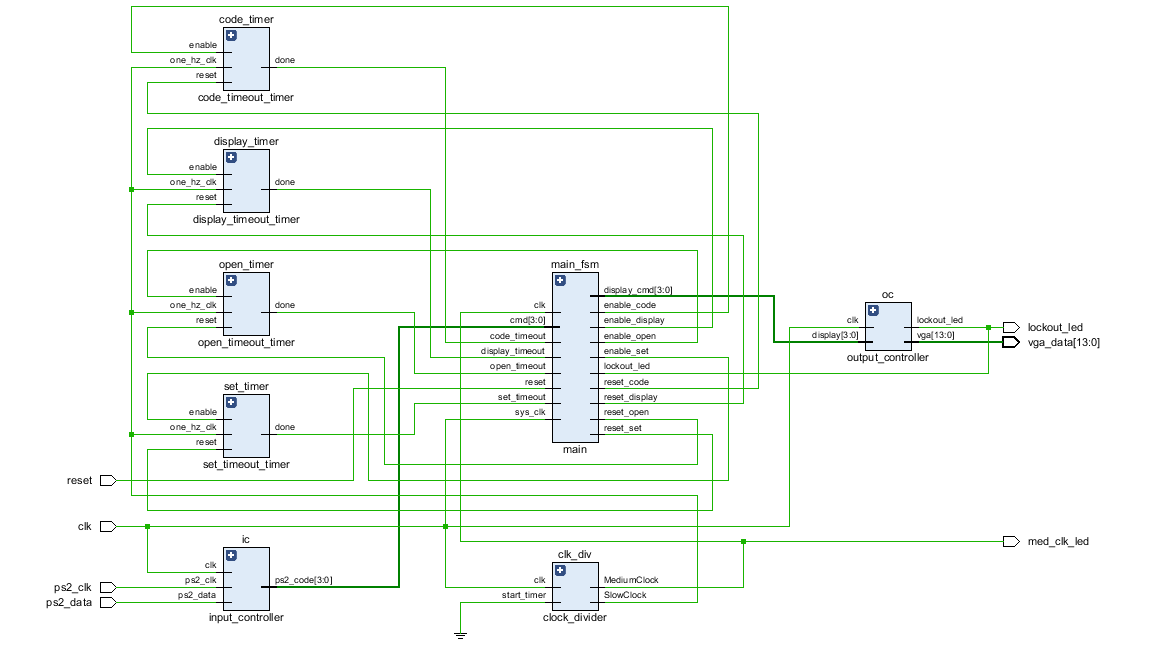
\includegraphics[width=\textwidth]{../docs/images/level1.png}
	\caption{\label{fig:level1}Level 1 System Diagram}
\end{center}
\end{figure}

The block diagram in Figure ~\ref{fig:level1} was updated in the course of my design process. The final level 1 diagram is shown in Figure ~\ref{fig:level1rev} below.

\begin{figure}[H]
\begin{center}
	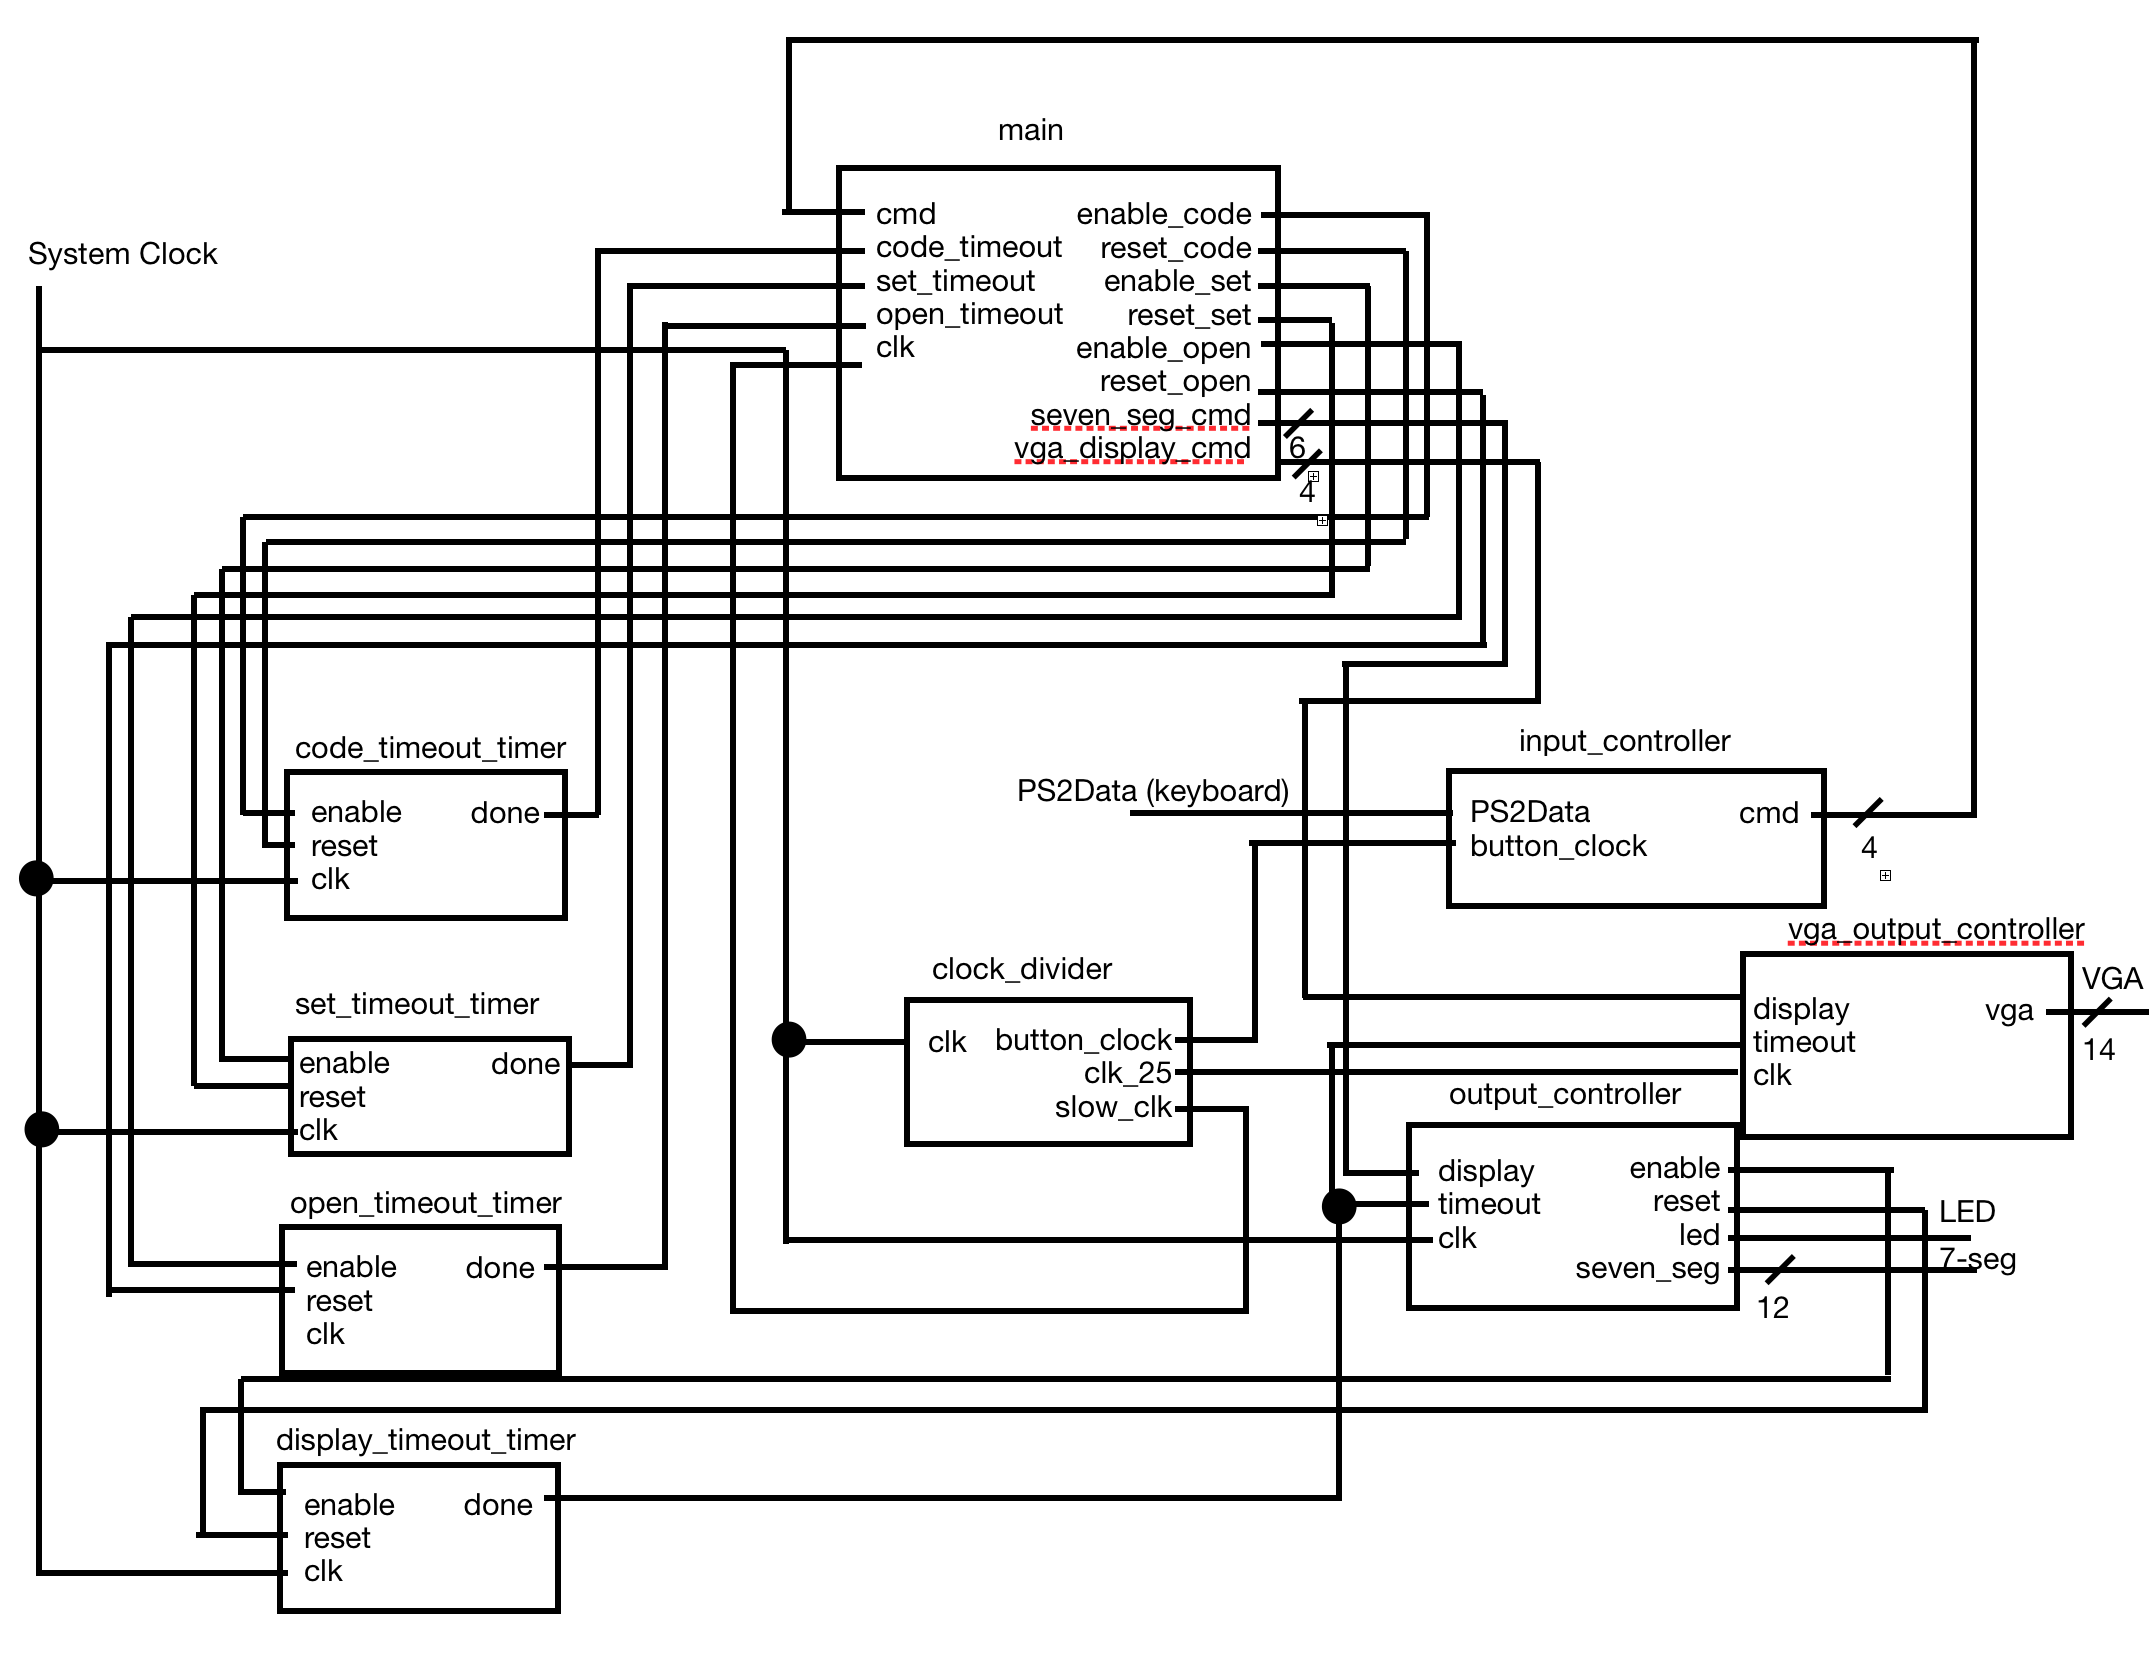
\includegraphics[width=\textwidth]{../docs/images/level1revised.png}
	\caption{\label{fig:level1rev}Revised Level 1 System Diagram}
\end{center}
\end{figure}

\section{Functional Specification}

\subsection{Initial Setup}

Initially, the system will have no code programmed. The user may program a code by pressing '+' to enter set mode. The user should then enter a 6-digit numeric code on the keypad and then press the '+' button again. This will exit set mode and save the code.

If the user enters more or less than 6 digits, or any non-numeric characters, the '+' key will cause the currently entered code to be cleared so the user may start setting again. If the code is cleared in this way, the VGA display should show "clr".

\subsection{Unlocking the Lock}

The keypad will be read every 0.25 seconds. The user should enter 6 numeric characters. As each character is entered,  it will be displayed on the VGA display. After 6 characters are read, the system will display "Open" on the VGA display if the correct code was entered, and "Err" if it was not.

The lock will remain unlocked for 15 seconds, and then the message will disappear and the system will be locked.

\subsection{Changing the Code}

To change the code after initial setup, the user must first enter the code. Then, while "OPEN" is displayed, press the '+' button to enter set mode.

Then, enter a 6-digit numeric code on the keypad and press the '+' button again. This will exit set mode and save the code.

If the user enters more or less than 6 digits, or any non-numeric characters, the '+' key will cause the currently entered code to be cleared so the user may start again. If the code is cleared in this way, the VGA display should show "clr".

\subsection{Display Timeout}

All messages on the VGA display, except for the "OPEN" message, will disappear after 2 seconds, or until a new character is entered, whichever comes first.

\subsection{Code Input Timeout}

If less then 6 digits are entered, they will be cleared after 20 seconds of no input from the user.

\subsection{Lockdown Mode}

If the incorrect code is entered 3 time, the system will enter lockdown mode. This will activate an LED indicator and the system will not unlock until its power is cycled.

\section{Development Milestones}

\subsection{Gantt Chart}

\begin{figure}[H]
\begin{center}
	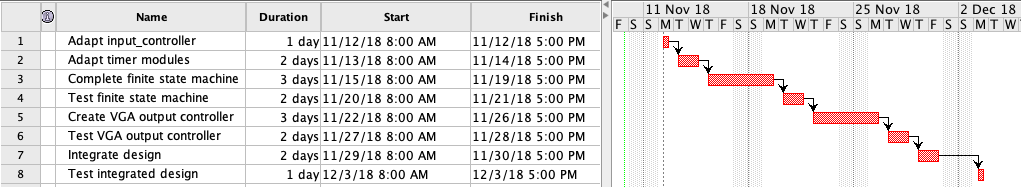
\includegraphics[width = \textwidth]{../docs/images/Timeline.png}
	\caption{\label{fig:gantt} Digital Lock development Gantt Chart}
\end{center}
\end{figure}

\section{Pitfalls}

While I was able to integrate the system timing well enough to move the state machine through multiple states, it jumped through unexpected states in a way that I did not expect. However, during the simulation phase, I was able to successfully navigate through states using ModelSim without jumping or errors. Therefore, I believe my biggest pitfall for this project was my inability to accurately identify the timing of my input controller. For most of my working time, I was working with the assumption that my debouncer module was working well enough to prevent false inputs from the input controller, but I now believe that to be false.

During project 1, I spent too much time on my output controller before integrating my input controller and main finite state machine. For this project, I intended to correct this, by integrating my input controller and main finite state machine before diving deep into my output controller. Unfortunately, this course correction slightly overcorrected, and my inability to complete the input controller integration led to me not producing a viable output controller.

\section{Achievements}

My most significant achievement for this project was the fully-functioning finite state machine that I was able to test in simulations. While it didn't time correctly with my input, the successful implementation of this finite state machine was no small feat, and testing it successfully and thoroughly was an accomplishment all its own.

Additionally, I feel that I verified to the best of my ability that the debouncer did the best it could with my input controller signal. While the signal still did not time up right with my state machine, I am confident that I successfully retrieved the cleanest possible signal, I just missed something with handling it after that point.

\section{Conclusion}

This project was a significant challenge, and it was very gratifying to work on a project that could easily be a real engineering challenge completed in industry. While I wasn't able to complete a fully functioning product, I believe that the planning and troubleshooting experience I gained in this project, as well as the technical knowledge about VHDL and FPGAs, will make it easier for me to approach similar problems in the workplace.

\pagebreak

\textbf{Appendices}

\begin{appendices}

\section{Clock Divider Code}

\lstinputlisting[language=Octave]{../src/clock_divider.vhd}

\section{Code Timeout Timer Code}

\lstinputlisting[language=Octave]{../src/code_timeout_timer.vhd}

\section{Display Timeout Timer Code}

\lstinputlisting[language=Octave]{../src/display_timeout_timer.vhd}

\section{Open Timeout Timer Code}

\lstinputlisting[language=Octave]{../src/open_timeout_timer.vhd}

\section{Set Timeout Timer Code}

\lstinputlisting[language=Octave]{../src/set_timeout_timer.vhd}

\section{Debouncer Code}

\lstinputlisting[language=Octave]{../src/debouncer.vhd}

\section{Input Controller Code}

\lstinputlisting[language=Octave]{../src/input_controller.vhd}

\section{Main Finite State Machine Code}

\lstinputlisting[language=Octave]{../src/main.vhd}

\section{Seven Segment Output Controller Code}

This output is strictly for debugging purposes. It shows the current state of the system on the seven-segment display.

\lstinputlisting[language=Octave]{../src/output_controller.vhd}

\section{Top Level Code}

\lstinputlisting[language=Octave]{../src/digital_lock.vhd}

\end{appendices}

\pagebreak

\begin{thebibliography}{9}

\bibitem{embedthoughts}
  Driving a VGA Monitor Using an FPGA, \\
  Embedded Thoughts, \\
  \verb!https://embeddedthoughts.com/2016/07/29//! \\
  \verb!driving-a-vga-monitor-using-an-fpga!
 
\bibitem{larson}
  VGA Controller, \\
  Scott Larson, \\
  EE Wiki, \\
  \verb!https://www.digikey.com/eewiki/pages/! \\
  \verb!viewpage.action?pageId=15925278!
\end{thebibliography}

\end{document}